\section{本文问题、证据层与阅读路径}\label{sec:1-5}

前四节从谱线的多重解释出发，界定了微观核电荷四极形状的量子描述层次，回顾了早期几何模型到微观自洽响应的发展历程，并建立了跨六个典型质量区的条件比较坐标。从实验室坐标系中测量的离散谱学信号，走向原子核内部的空间电荷分布与三维集体运动，是一条经过多级物理抽象与实验截断约束的反演路径。

本节归纳全书的核心问题，阐明实验直接报告、采用外部输入、模型计算与本稿推导之间的证据边界，说明竞争假说的可证伪性检验准则，并给出贯穿全书五章的论证逻辑与阅读路径。

\subsection{从实验室矩阵元到内禀形状与取向的反演链条}\label{sec:1-5-1}

在低能核结构与在束 $\gamma$ 谱学实验中，探测系统直接记录的物理事件是数字化脉冲波形、沉积能量通道与瞬变符合时间戳。为了从这些直接信号推断内部电荷形状与空间取向，数据分析通常经历逐级深入的处理链条：
\begin{enumerate}
    \item \textbf{直接信号到计数与符合}：通过探测器能量线性与全能峰效率校准，对多探测器符合事件进行时间对准与偶然符合扣除，构建对称或非对称符合矩阵，建立核能级纲图拓扑与初末态连接关系。
    \item \textbf{激发态特性与采用输入}：利用多普勒频移衰减法（DSAM）或反冲距离多普勒法（RDDS）测定激发态平均寿命 $\tau$；通过实验测得的光子分支比与方向角关联（DCO）或线偏振度提取多极混合比 $\delta(E2/M1)$。在将寿命映射为绝对跃迁几率 $B(E2)$ 与 $B(M1)$ 时，往往需要采用外部输入的内转换系数 $\alpha_{\text{IC}}$（通常来自原子电子结构计算或评价数据，如第~5.9~节所述），或沿用先前实验的薄靶弱分支数据。
    \item \textbf{旋转不变量与内禀形状映射}：在多步库仑激发实验中，测量的布居截面网络经解耦提取出对角与非对角电四极约化矩阵元。利用 Kumar--Cline 旋转不变量方法~\cite{cline-1986-nuclear-shapes-coulomb-excitation}，矩阵元二次与三次标量缩并给出的标量期望值 $q_2 = \langle Q^2 \rangle$ 与 $q_3 = \langle Q^3 \cos(3\gamma) \rangle$ 能在模型无关的意义下约束电荷四极关联矩。但将这些标量矩进一步反解为内禀椭球形变参数 $(\beta, \gamma)$ 时，必须引入具体几何波包假设与有限激发态截断修正，因而不等同于连续空间电荷密度的无条件几何断层扫描。
    \item \textbf{候选集体动力学与取向模式}：非轴对称性（$\gamma \ne 0^\circ, 60^\circ$）是激发三维空间取向动力学（如摆动模式与手征对称性）的候选几何条件。当转动惯量沿不同主轴产生分离时，体系可能发生绕主轴进动的摆动激发~\cite{bohr-mottelson-1953-collective-individual-original}；当费米面附近的高 $j$ 价粒子、价空穴与中轴转动的核芯角动量相互垂直形成非共面几何时，体系在内禀参考系中破缺时间反演与特定主轴旋转的联合对称性 $\mathcal{T}\mathcal{R}_y(\pi)$，在微观波函数隧穿恢复后可能展现出同宇称的手征双重带候选~\cite{petrache-2006-near-degenerate-chiral-misinterpretation}。非轴对称与非共面参考构型是否能在实际能谱中建立，必须取决于具体轨道占据、相互作用响应以及波函数的动力学特征，不能仅凭唯象几何势能极小断言真实转动模式的存在。
\end{enumerate}

这一链条表明：从实验室测量走向微观取向动力学，每一步都包含明确的物理映射与适用条件。

\subsection{证据分层、可证伪性与竞争解释的检验规范}\label{sec:1-5-2}

为了保持学术论证的受控与客观，本论文将物理主张与数据依据划分为四个明确的证据层次，并严格区分直接测量与依赖关系：
\begin{enumerate}
    \item \textbf{实验直接报告及分析依赖}：指在束测量中可直接复现的经验报告，包括离散能级峰位、符合强度、线形多普勒衰减曲线、角关联比值等，以及由这些原始数据在明确谱学假定下提取的能级能量与寿命。
    \item \textbf{采用外部输入与共享依赖}：指在反演过程中引用的先前文献数据，包括弱退激分支比、外部测量的多极混合比 $\delta$、评价数据库的内转换系数 $\alpha_{\text{IC}}$、原子质量及邻核能级参数。在评估结论独立性时，必须将这些采用量显式隔离，避免将共享同一历史输入的多次推导误计为多项独立实验支持。
    \item \textbf{作者解释与模型计算}：指文献作者提出的物理图像以及微观自洽平均场、粒子---转子模型或壳模型计算的理论输出（如极小形变、推导位能面、理论过渡四极矩或单粒子组态赋值）。模型计算是理解机制的重要工具，但理论预言绝不能冒充实验观测事实。
    \item \textbf{本稿条件推导与综合分析}：指本论文在对齐符号规范、核对中间态截断不确定度、检查相对相位以及系统对比竞争模型预言时给出的推导结论与论证边界。
\end{enumerate}

在核结构动力学分析中，表观能谱吻合或局域近简并往往容许机制迥异的模型解释。为了打破解释简并，科学分析不能依赖单一指标作绝对裁决，而必须针对具体候选模型，系统比较多项额外且尽量独立的可观测预言：
\begin{itemize}
    \item \textbf{摆动激发与竞争模式}：奇 $A$ 核中伴随基态带出现的近简并侧带，既可能是准粒子绕非主轴进动的横向摆动（TW）或纵向摆动（LW）~\cite{campaign-g07-gorgen-2004-163lu-quadrupole-moments}，也可能源于倾斜轴进动（TiP）或准粒子与 $\gamma$ 振动核芯的四极声子耦合。区分这些模式不能依赖固定主轴的先验设定，而需综合比较带间与带内绝对跃迁几率比值 $B(E2)_{\text{out}}/B(E2)_{\text{in}}$、$B(M1)_{\text{out}}/B(E2)_{\text{in}}$ 随自旋的演化趋势、转动频率平面顺排角动量特征以及核芯微观响应。
    \item \textbf{手征双重带与组态解混合}：奇奇核中两条同宇称能带的局域能量近简并，本身并不构成空间手征取向的充分证据。多准粒子能级交叉与组态解混合同样可以在有限自旋窗口产生表观相近的能级间距~\cite{petrache-2006-near-degenerate-chiral-misinterpretation}。检验手征物理假说需要进一步比对两带内禀四极矩是否具有共同的三轴核芯特征、带间 $M1$ 与 $E2$ 强度的交错规律以及高自旋端顺排角动量的演化行为。
    \item \textbf{刚性三轴形变与动态 $\gamma$ 软性}：由二次与三次旋转不变量提取的有效三轴角 $\gamma_{\text{eff}}$，既可以来自具有深势阱的刚性三轴极小（Davydov--Filippov 刚性转子模型），也可以源于沿 $\gamma$ 方向势能平坦的量子振动弥散（Wilets--Jean 软核模型）~\cite{poves-2020-limits-assigning-nuclear-shape}。对这一物理机制的鉴别，需要结合四阶四极标量涨落宽度 $\Delta A/\langle \hat{A} \rangle$、能谱交错函数 $S(I)$ 以及高激发态退激分支网络开展多方位比较。
\end{itemize}

客观的科学裁决只能建立在实验测量的不确定度边界、受控的数学推导与竞争假说对留出观测的综合检验之上。

\subsection{论文逻辑架构与各章先修回扣关系}\label{sec:1-5-3}

为了越过表观拟合的多重解释，全篇论文围绕微观多体机制、唯象动力学模型与在束实验反演技术展开，各章聚焦一个核心读者问题并形成环环相扣的论证闭环：

\begin{figure}[htbp]
\centering
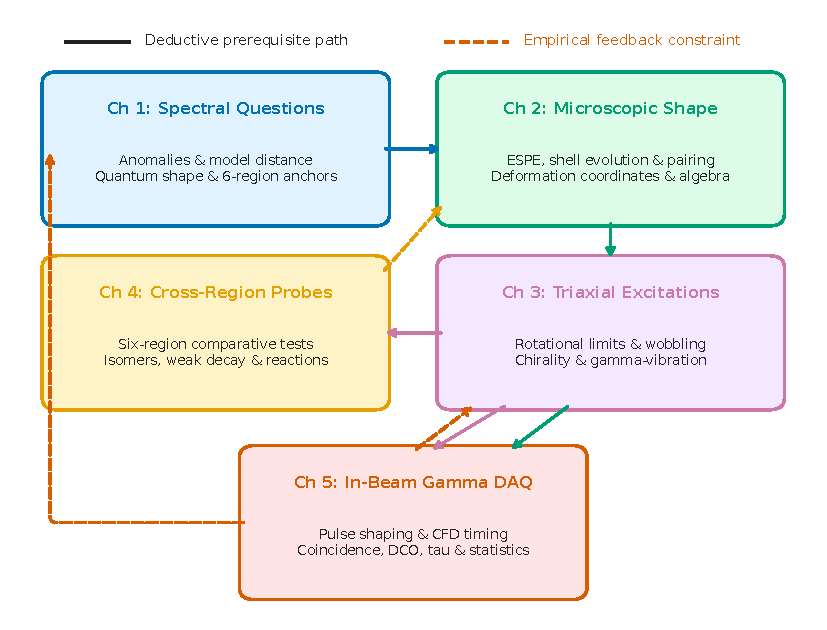
\includegraphics[width=.92\textwidth]{Img/chapter-dependency.pdf}
\caption{全篇论文五章逻辑架构与论证依赖关系概念示意图。从第1章提出谱学反演核心问题出发，经微观理论基础（第2章）、三轴取向动力学（第3章）、六区经验检验（第4章）与在束实验技术链（第5章）闭环展开。}\label{fig:chapter-dependency}
\end{figure}

\begin{itemize}
    \item \textbf{第 1 章：从谱线提出问题}（本章）\\
    \textit{读者核心问题}：在束实验记录的离散谱线为什么容许多种动力学解释？微观核形状与三维取向应在何种量子力学层次上定义？\\
    \textit{章间承接}：本章澄清了一阶实验室静矩与内部四极关联的区别，回顾了早期几何统一模型到微观响应的发展脉络，建立了六个质量区的比较坐标与证据分层规范，为第~2~章奠定微观哈密顿量与张量代数基础。

    \item \textbf{第 2 章：从核子到量子形状}\\
    \textit{读者核心问题}：微观核子之间的有效相互作用、费米面轨道占据与配对关联，如何自洽涌现出具有好角动量的量子态、内部四极关联与集体惯量？\\
    \textit{章间承接}：系统建立不可约球张量代数、有效单粒子能量（ESPE）单极演化、Bogoliubov 准粒子变换、五维四极几何测度与 Thouless--Valatin 动力学转动惯量响应，将抽象的形状坐标落实为微观波函数可计算量，为第~3~章处理三轴核的空间取向运动提供理论工具。

    \item \textbf{第 3 章：三轴及耦合激发}\\
    \textit{读者核心问题}：当微观势面涌现出三轴非轴对称形变时，核体系会展现出哪些特征空间取向模式，如何从电磁跃迁特征甄别这些模式？\\
    \textit{章间承接}：推导非轴对称转子稳定转轴的惯量排序判据与小振幅摆动激发频率，分析高自旋准粒子顺排对横向/纵向摆动的控制机制；研究三维非共面角动量手征几何的波函数隧穿与电磁选择定则；推导形状模与取向模耦合以及反射不对称八极关联，建立可证伪的联合预言矩阵，为第~4~章的跨核区实测比较提供理论判据。

    \item \textbf{第 4 章：六区的条件比较与两翼探针}\\
    \textit{读者核心问题}：第~2~章与第~3~章建立的微观形状与三轴动力学判据，在具体核素的激发态实验现实中表现出怎样的共性与个性？\\
    \textit{章间承接}：以 $A\approx 130$ 质量区为核心锚点，针对具体的核素、激发态能级与组态，比较 $A\approx 60$（$^{64}\mathrm{Ge}$ 敲出反应寿命与理论四极矩列）、$A\approx 80$（$^{74,76}\mathrm{Kr}$ 多步库仑激发两态混合）、$A\approx 100$（$^{98}\mathrm{Zr}$ 结构演化与外部分支比采用）、$A\approx 160$（$^{163}\mathrm{Lu}$ 摆动候选绝对跃迁强度与采用依赖）以及 $A\approx 190$（$^{182\text{--}188}\mathrm{Hg}$ 库仑激发对角项误差边界）的实验测量现实；讨论反射---手征耦合候选核；分析同核异能态对微观波函数的选择机制；结合 Gamow--Teller 与禁戒跃迁等弱相互作用探针研究壳演化；最终引出支撑这些物理量测定的在束实验测量源头。

    \item \textbf{第 5 章：完整实验技术链}\\
    \textit{读者核心问题}：前述各章所依赖的能级纲图、激发态寿命、混合比及绝对跃迁几率，最初是如何从重离子核反应与探测器原始信号中被反演与标定的？\\
    \textit{章间承接}：系统回溯核反应布居截面、高纯锗阵列探测响应、数字化脉冲梯形成形滤波与 CFD 定时、符合拓扑分析与能级建立、角分布与偏振联合似然反演、DSAM/RDDS 寿命测定以及绝对跃迁几率误差传播。通过揭示数据生成的底层物理与统计不确定度，完成全书从实验谱线到微观物理、再回到实验验证的完整闭环。
\end{itemize}

需要明确说明：本章作为博士论文的前置导读与研究框架确立，全部内容均建立在已有公开发表文献与经典核物理理论之上，旨在理清推断逻辑与论证边界；本章不包含未经验证的个人实验成果，所涉及的代表性谱学测量均归属于原引证实验。
